\section{Linear Basis Function Regression} \label{sec:prob2}
In this section, we consider two types of linear basis functions for regression: polynomial and cosine. We try different model complexities to compare the performance.

\subsection{Part 1}
At first, we don't know the true basis for our dataset, and want to try \textit{polynomial} models of different complexities.
Given an array of data points $X$ and a vector $Y$ of values, a simple polynomial basis,
\begin{equation}
\phi_0(x) = 1, \phi_1(x) = x, ..., \phi_M(x) = x^M\label{eq:polynomial_basis}
\end{equation}
is applied to the $X$ points, for several values of M.

\cref{fig:2_3} shows the data as black circles, and the true function from which the data is generated in green.
The orange in each subplot is the polynomial basis model, and blue is a cosine model (described in [pt 4]).
(The other curves will be described later.)
The model complexity is insufficient to capture the variation in the data with M=0~\cref{fig:2_3} (leftmost) since the model is a line with zero slope.
For M=1, the linear-plus-constant basis, is still insufficient to capture the concave structure in the dataset.
M=2 seems like a good choice visually, as it does not intersect every data point exactly but captures the concave shape.
On the rightmost plot, M=10 overfits the data, which means it evaluates exactly to the correct values in the dataset but does not look like the smooth, green line from which the data was generated.


\begin{figure}
	\centering
	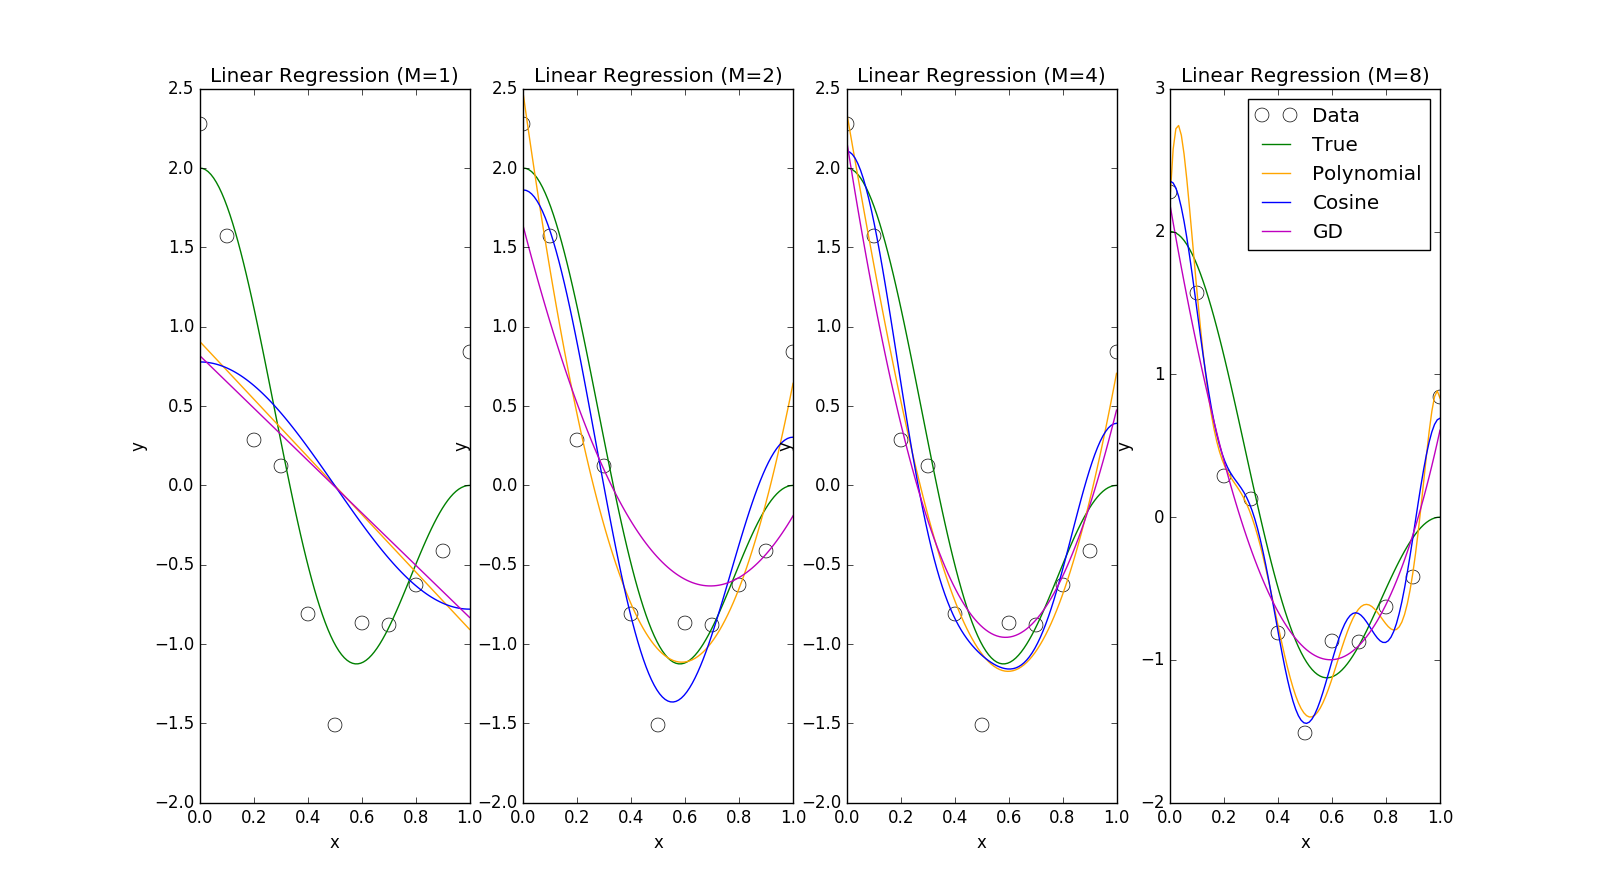
\includegraphics [trim=0 0 0 0, clip, angle=0, width=0.8\columnwidth,
	keepaspectratio]{figures/2_3}
	\caption{For different M values (1,2,4,8) a polynomial (orange) and cosine (blue) basis is used to fit the dataset (black circles). The true function used to generate the data is shown in green in each plot. For low model complexity (left plot), the model doesn't capture the variation in the data. For high model complexity (right plot), the model overfits the data. Also shown is Batch GD (magenta) and SGD (black) on SSE.}
	\label{fig:2_3} 
\end{figure}

\subsection{Part 2}
Next, we implemented a calculation sum-of-squares error (SSE) (Bishop 3.26):
\begin{equation}
E(w) = \sum_{i=1}^{N} (y^{(i)}-w^T\cdot \phi(x^{(i)}))^2
\label{eq:sse}
\end{equation}
and its gradient.
To confirm that the analytic gradient is close to the approximate gradient, we measured the norm difference between the two methods for a single run of Batch GD.
The average norm error (over 100 iterations) was 0.0119 with $\delta x = 0.01$.
This implies the gradient was likely implemented correctly.

\subsection{Part 3}
We then tried Batch GD on the SSE function.
It was sensitive to the intial guess, and would not always converge to a good solution if initial guess was far off.
This could be because the SSE function is more complicated than the simple negative gaussian and quadratic bowl from the first problem.
Similar to previous experience with GD, if learning rate was too high, it would diverge and if learning rate was too low, the parameters would not change enough between iterations.

\cref{fig:2_3} shows the Batch GD solutions compared with other methods.
Batch GD (magenta) and does not seem to overfit the data as much at high model complexity (right side), but does not capture the trend as well as regression methods (left-middle) for low complexity.
The Batch GD parameters used across models are $\epsilon=10^{-3}$, $\alpha=0.01$, and $n_{iters}=100$.

For SGD (black in~\cref{fig:2_3}) the performance is similar to Batch GD.
It also depends on initial guess being close to final answer.
The SGD parameters used across models are $\epsilon=10^{-8}$, $\tau_0=10^8$, $k=0.6$, $n_{iters}=10000$.
The convergence limit for SGD had to be set lower than in Batch GD to ensure randomness does not cause the algorithm to terminate very early.
Note there is a scaling factor (dataset size) between the two GD algorithm's $n_{iters}$ in our definition which explains the large difference.
The M=2 SGD solution does not look very accurate.
Presumably this particular model's parameters could be adjusted for good performance but it demonstrates the brittleness as is.

\subsection{Part 4}
Since we know the dataset was actually generated from a sum of cosines, a set of cosine basis functions should lead to a better fit than polynomials.
The cosine basis functions with intercept term $\phi_0$ are:
\begin{equation}
	\phi(x)=(1, cos(\pi x), cos(2\pi x), ... , cos(M\pi x))
\end{equation}
Again referring to~\cref{fig:2_3}, there is a similar trend (in both polynomial and cosine bases) of underfitting and overfitting for small and large model complexities, respectively.
The M=2 cosine model fits the data pretty well, similar to the M=2 polynomial.
This is no coincidence, because the data was generated from a pair of cosines (M=2), specifically $y = cos(\pi x) + cos(2\pi x)$.

The actual values of the weight vector's elements can also be compared to the true function in~\cref{table:w}.
The M=2 case does not give the exact same values as the actual function's coefficients, but this could possibly be improved using regularization, more data, data with lower noise, or removing the bias ($w_0$) term.
With the complex model (bottom row, M=8), the high frequency components (7, 8) have very low magnitude.

\begin{table*}[t]
  \centering
  \caption[]{Cosine Basis Function Weights}
	\begin{tabular}{|p{1cm}||p{1cm}|p{1cm}|p{1cm}|p{1cm}|p{1cm}|p{1cm}|p{1cm}|p{1cm}|p{1cm}|}
	 \hline
	 \multicolumn{10}{|c|}{Cosine Basis Function Weights} \\
	 \hline
	 M & 0 & 1 & 2 & 3 & 4 & 5 & 6 & 7 & 8 \\
	 \hline\hline
	 Actual & 0 & 1 & 1 & - & - & - & - & - & - \\
	 1 & 0.0 & 0.78 & - & - & - & - & - & - & - \\
	 2 & -0.11 & 0.78 & 1.19 & - & - & - & - & - & - \\
	 4 & -0.13 & 0.76 & 1.16 & 0.09 & 0.22 & - & - & - & - \\
	 8 & -0.15 & 0.77 & 1.1 & 0.1 & 0.16 & -0.05 & 0.38 & 0.01 & 0.03  \\
	 \hline
	\end{tabular}
	%\caption*{Effect on ahsaseefah. }
	\label{table:w}
\end{table*}

